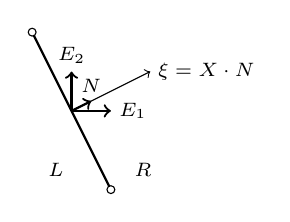
\begin{tikzpicture}[scale=0.5]
  % \draw (10.,0.) -- (12.,6.) ;
  % \draw[fill=white] (9.85,0.1) circle (0.1) node [left] {$1$};	
  % \draw[fill=white] (10.2,-0.0) circle (0.1) node [right] {$2$};	
  % \draw[fill=white] (11.85,6.1) circle (0.1) node [left] {$4$};	
  % \draw[fill=white] (12.2,6) circle (0.1) node [right] {$3$};	
  % \draw[black] (9.85,0.1) circle (0.1) node [left] {$1$};	
  % \draw[black] (10.2,-0.0) circle (0.1) node [right] {$2$};	
  % \draw[black] (11.85,6.1) circle (0.1) node [left] {$4$};	
  % \draw[black] (12.2,6) circle (0.1) node [right] {$3$};	
  % \draw[->,very thick] (11.,3.) -- (12,3 -1/3) node [right,below] {$X_N$}; 
  % \node at (8,3.5) {$\Ucb_{X_N^-} = \frac{\Ucb_1 + \Ucb_4}{2}$}; \node at (14.5,3.5) {$\Ucb_{X_N^+} = \frac{\Ucb_2 + \Ucb_3}{2}$};
  \begin{scriptsize}
    \draw[thick] (0.0,0.0) -- (-2,4.) ;
    \draw[->,thick] (-1,2.) -- (-1,3.) node [above] {$\vect{E}_2$};
    \draw[->,thick] (-1,2.) -- (-.,2.0) node [right] {$\vect{E}_1$};
    \draw[->] (-1,2) -- (1.,3) node [right] {$\xi= \vect{X}\cdot \vect{N} $};
    \draw[->,thick] (-1,2.) -- (-0.5,2.25) node [right,above] {$\vect{N}$};
    \node[left] at (-1,0.5) {$L$};
    \node[right] at (.4,0.5) {$R$};
    \draw [fill=white] (0,0) circle (0.1);
    \draw [fill=white] (-2,4) circle (0.1);
    \end{scriptsize}
\end{tikzpicture}

%%% Local Variables:
%%% mode: latex
%%% TeX-master: "../../presentation"
%%% End:
